\section{Laufzeitsicht (FA)}
Nachfolgend sollen die dynamischen Aspekte des Systems dargestellt werden. Dabei wird aufgezeigt, wie die unterschiedlichen Teile der Software bei den grundlegenden Funktionen der Software zusammen spielen.

\subsection{Anlegen eines Schülers}
\begin{figure}[H]
	\centering
	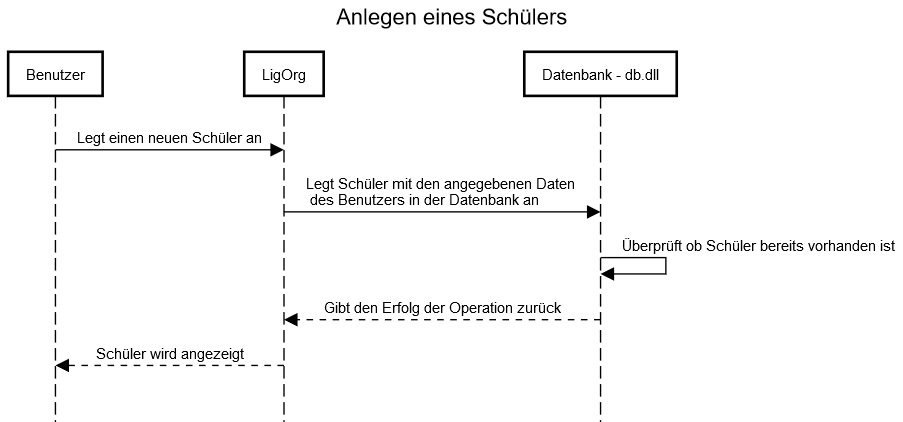
\includegraphics[width=0.80\textwidth]{figures/laufzeit/newstudent.png}
	\caption{Ablauf für das Anlegen eines Schülers}
	\label{fig:newstudent}
\end{figure}
Zunächst gibt der Benutzer die benötigten Daten in die Eingabemaske ein und bestätigt in der Benutzeroberfläche, dass er den neuen Schüler anlegen will. Daraufhin ruft die Hauptanwendung LibOrg die entsprechende Funktion der Datenbank-API auf, welche in der Datenbank den Schüler mit den vom Nutzer angegebenen Daten anlegt. Hier wird überprüft, ob der Schüler eventuell schon vorhanden ist. Nach der Ausführung der oben genannten Funktion der Datenbank-API, wird der Hauptanwendung mitgeteilt, ob der Schüler erfolgreich angelegt wurde. Wenn dies der Fall ist wird der angelegte Schüler fortan für den Benutzer angezeigt.

\subsection{Löschen eines Schülers}
\begin{figure}[H]
	\centering
	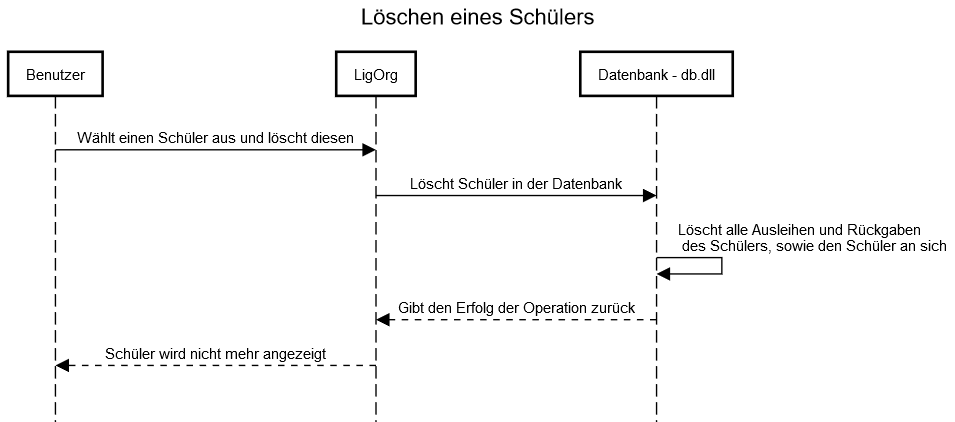
\includegraphics[width=0.80\textwidth]{figures/laufzeit/removestudent.png}
	\caption{Ablauf für das Löschen eines Schülers}
	\label{fig:removestudent}
\end{figure}
Hier wird vom Benutzer der zu löschende Schüler ausgewählt, daraufhin erscheint eine Sicherheitsabfrage, ob der Schüler wirklich gelöscht werden soll (die Sicherheitsabfrage weist auch darauf hin, ob ein Schüler noch offene Ausleihen besitzt). Wird dies bestätigt, ruft die Hauptanwendung die entsprechende Funktion der Datenbank-API auf mit den Daten des ausgewählten Schülers. Innerhalb der Datenbank werden zunächst alle Ausleihen und Rückgaben dieses Schülers gelöscht. Daraufhin wird auch noch der Schüler gelöscht. Der Hauptanwendung wird das Ergebnis der Operation mitgeteilt und der Schüler wird fortan nicht mehr angezeigt.

\subsection{Anlegen eines Buches}
\begin{figure}[H]
	\centering
	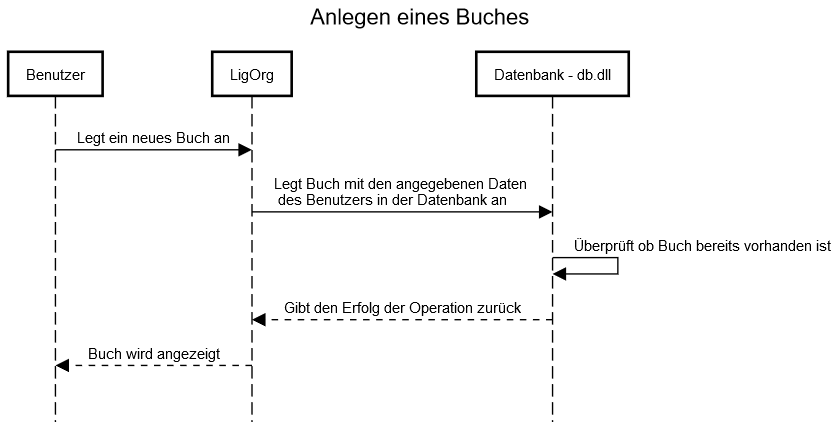
\includegraphics[width=0.80\textwidth]{figures/laufzeit/newbook.png}
	\caption{Ablauf für das Anlegen eines Buches}
	\label{fig:newbook}
\end{figure}
Anfänglich gibt der Benutzer die nötigen Daten des neuen Buches in die Eingabemaske ein und bestätigt die Erstellung des Buches. Die Hauptanwendung gibt die Daten an die entsprechende Funktion der Datenbank-API weiter, diese legt das Buch in der Datenbank an. Dabei wird überprüft, ob das Buch bereits vorhanden ist. Die Datenbank-API gibt das Ergebnis der Operation an die Hauptanwendung zurück und das neue Buch wird bei Erfolg angezeigt.

\subsection{Löschen eines Buches}
\begin{figure}[H]
	\centering
	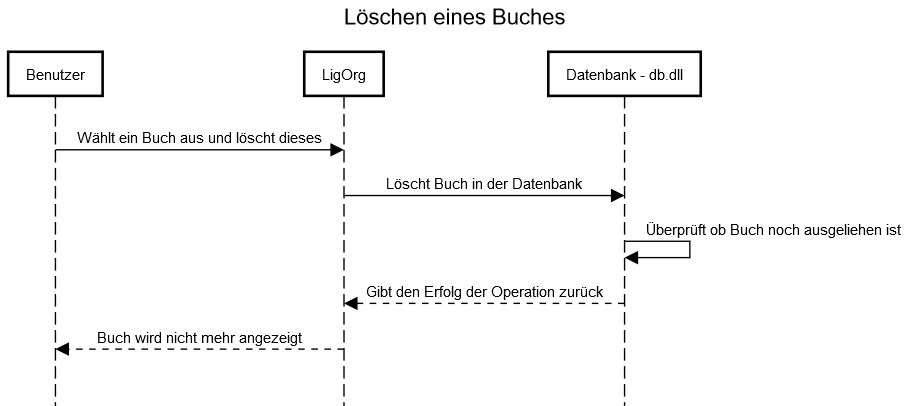
\includegraphics[width=0.80\textwidth]{figures/laufzeit/removebook.png}
	\caption{Ablauf für das Löschen eines Buches}
	\label{fig:removebook}
\end{figure}
Der Benutzer wählt das zu löschende Buch aus und bestätigt die Operation durch eine Sicherheitsabfrage. Die Hauptanwendung gibt daraufhin die Daten des ausgewählten Buches an die Datenbank-API weiter, welche überprüft, ob das ausgewählte Buch noch von Schülern ausgeliehen ist. Ist dies der Fall, kann das Buch nicht gelöscht werden. Ansonsten wird der Erfolg der Operation an die Hauptanwendung zurückgegeben und das Buch wird nun nicht mehr angezeigt.

\subsection{Ausleihen eines Buches}
\begin{figure}[H]
	\centering
	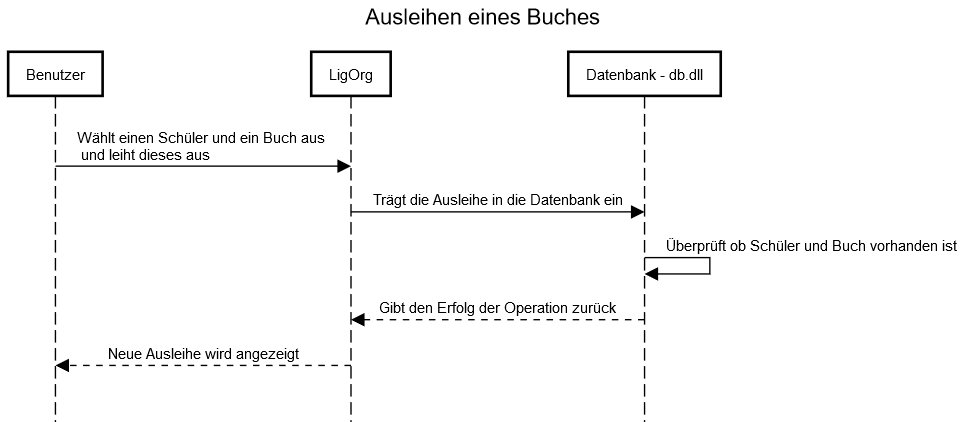
\includegraphics[width=0.80\textwidth]{figures/laufzeit/lending.png}
	\caption{Ablauf für das Ausleihen eines Buches}
	\label{fig:lending}
\end{figure}
Um eine Ausleihe anzulegen, muss der Benutzer zunächst ein Buch und einen Schüler auswählen und per Benutzeroberfläche die Ausleihe eintragen. Diese Daten werden von der Hauptanwendung an die Datenbank-API übergeben. Hier wird vorerst überprüft, ob der ausgewählte Schüler und das Buch vorhanden sind. Ist dies der Fall, wird die Ausleihe in der Datenbank eingetragen. Das Ergebnis der Operation wird an die Hauptanwendung zurückgegeben, woraufhin bei Erfolg fortan die Ausleihe in der Benutzeroberfläche angezeigt wird.

\subsection{Zurückgeben eines Buches}
\begin{figure}[H]
	\centering
	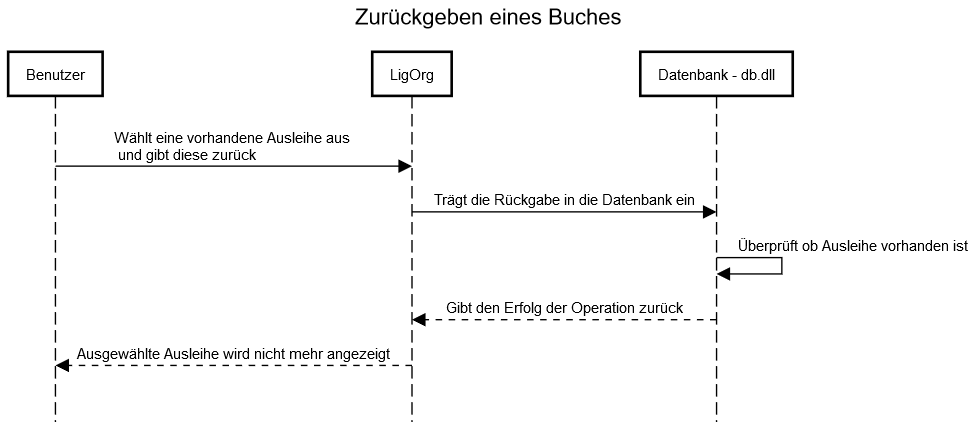
\includegraphics[width=0.80\textwidth]{figures/laufzeit/giveback.png}
	\caption{Ablauf für das Zurückgeben eines Buches}
	\label{fig:giveback}
\end{figure}
Bei dieser Operation muss der Benutzer eine bestehende Ausleihe auswählen und diese per Benutzeroberfläche zurückgeben. Die Daten der ausgewählten Ausleihe werden an die Datenbank-API übergeben. Hier wird überprüft, ob die ausgewählte Ausleihe wirklich existiert. Daraufhin wird eine Rückgabe für die entsprechende Ausleihe eingetragen. Nun wird der Erfolg der Operation zurückgegeben und die vom Benutzer ausgewählte Ausleihe wird fortan nicht weiter angezeigt. 
